\documentclass[12pt, a4paper, oneside]{book}

%----- ALL THE JUICY PACKAGES -----%
\usepackage[T5]{fontenc} % Make it possible to copy accented characters from ouput files
% Since this is a Vietnamese document so I am using T5 here, if you are writing a pure English or whatever change it to T1
% Read more: https://tex.stackexchange.com/questions/664/why-should-i-use-usepackaget1fontenc
\usepackage[top=2cm, bottom=2cm, left=3cm, right=2cm, includeheadfoot]{geometry} % Set margin
\usepackage[utf8]{vntex} % VnTex is really good for Vietnamese document
\usepackage{mathptmx} % About the same as Times New Roman font
\usepackage{indentfirst} % Indent the first paragraph of sections
\usepackage{fancyhdr} % For fancy headers and footers
\usepackage{graphicx} % Enhanced support for graphics (DRAW STUFF)
\usepackage{tikz} % Create PostSscript and PDF graphics (DRAW MORE STUFF)
\usepackage{setspace} % Set custom space between lines
\usepackage[unicode]{hyperref} % Hypertext support, useful for making bookmarks and click-able hyperlinks
\usepackage[perpage]{footmisc} % Footnote restart everypage
\usepackage{amsmath} % Nice math package
\usepackage{siunitx} % Handles basically all of the SI Units stuff
\usepackage{booktabs} % Beautify tables/tabular/tableau
\usepackage{enumitem} % Less spacing between items in itemize list, also can use a new env enumerate
\usepackage{longtable} % longtable, able to span multiples pages
\usepackage{multirow} % Multirow for tables
\usepackage{minted} % Code highlighting
\usepackage{multido}
\usepackage{./custom_package/dirtree/dirtree}

% Bibliography management: by default LaTeX uses Biblatex which werks (with an e)
% but if you cite documents with non-ascii stuff in it (or want to customize bibiography)
% then it's highly recommended to use biber backend
\usepackage[backend=biber, style=ieee, maxbibnames=3, minbibnames=1]{biblatex}
%\AtEveryBibitem{\printfield{labelnumber}.\addspace} % Numbers in the bib, use with authoryear or whatever

%----- CUSTOM COMMANDS -----
\setcounter{secnumdepth}{4} % This will number the subsubsection
%\setcounter{tocdepth}{4} % This will add subsubsection line to TOC
\renewcommand{\thesubsubsection}{\alph{subsubsection})} % Use a) b) c) in subsubsection
%\renewcommand{\arraystretch}{1.2} % More space between table lines
% See: https://tex.stackexchange.com/questions/248451/how-to-create-multiple-dotted-lines
\newcommand{\Pointilles}[1]{%
  \par\nobreak
  \noindent\rule{0pt}{1.5\baselineskip}% Provides a larger gap between the preceding paragraph and the dots
  \multido{}{#1}{\noindent\makebox[\linewidth]{\dotfill}\endgraf}% ... dotted lines ...
  \bigskip% Gap between dots and next paragraph
}
\renewcommand\listingscaption{Ví dụ}
\renewcommand\listoflistingscaption{Danh sách ví dụ}
\newminted[ccode]{c}{frame=lines, linenos, breaklines, breakanywhere, fontsize=\footnotesize} % format rust code

%----- SUB-SETTINGS PACKAGES AND GENERAL PAGES -----%
\usetikzlibrary{calc} % For calculating space to draw stuff
\usetikzlibrary{arrows, positioning, fit, shapes.geometric} % stuff needed for block diagram
\onehalfspacing % From setspace package
\addbibresource{uni.bib} % This is for biblatex
\setlength{\headheight}{20pt} % vertical associated with header of the page (fancyhdr)
\setlist{nosep} % This is used with enumitem package, less space separator between items in lists/enums

%----- SETTINGS FOR HEADERS AND FOOTERS -----%
% Read more: https://en.wikibooks.org/wiki/LaTeX/Customizing_Page_Headers_and_Footers
\pagestyle{fancy}
\fancyhf{}
\lhead{Thực tập tốt nghiệp - \csCompileTime}
\rhead{GVHD: TS. Trương Quang Vinh}
\cfoot{\thepage}

%----- SETTINGS FOR CONSTANTS COUNCILS + COMPILE TIME -----%
\newcommand{\csdeptname}{KHOA ĐIỆN ĐIỆN TỬ}
\newcommand{\csCouncil}{Khoa Điện Điện tử}
\newcommand{\csCty}{Công ty TNHH 3D Sao Vàng}
\newcommand{\csSupervise}{TS. Trương Quang Vinh}
\newcommand{\csReviewer}{TS. Nguyễn Văn A}
\newcommand{\crname}{BÁO CÁO THỰC TẬP TỐT NGHIỆP} % Thesis, report, whatever
\newcommand{\csCompileTime}{07/2020}

%----- SUB-SETTINGS FOR STUDENT NAMES -----%
\newcommand{\csSVone}{Vũ Đăng Khoa}
\newcommand{\csidSVone}{1611645}
%\newcommand{\csSVtwo}{Rudo2204}
%\newcommand{\csidSVtwo}{123456}

%----- BEGIN FRONTMATTER -----%
\begin{document}
\frontmatter

%----- BEGIN TITLEPAGE -----%
\newgeometry{top=2cm, bottom=3cm, left=3cm, right=2cm}
\begin{titlepage}
%----- DRAWING BORDERS OF TITLEPAGE -----%
\begin{tikzpicture}[remember picture, overlay]
\draw [line width=1pt]
    ($ (current page.north west) + (3.15cm,-2.15cm) $)
    rectangle
    ($ (current page.south east) + (-2.15cm,2.15cm) $);
\draw [line width=3pt]
    ($ (current page.north west) + (3cm,-2cm) $)
    rectangle
    ($ (current page.south east) + (-2cm,2cm) $);
\end{tikzpicture}

%----- TYPESETTINGS INFORMATION OF TITLEPAGE -----%
\begin{center}
\begin{large}
ĐẠI HỌC QUỐC GIA THÀNH PHỐ HỒ CHÍ MINH\\
TRƯỜNG ĐẠI HỌC BÁCH KHOA\\
\csdeptname\\
\end{large}
\textbf{--------------------  *  ---------------------}\\[1.2cm]
\includegraphics[scale=0.25]{images/LogoBK.png}\\[1.2cm]
%{\fontsize{15}{1}\selectfont \crname }\\[0.8cm]

%----- TYPESETTINGS INFORMATION OF TITLE -----%
{\fontsize{24}{1}\selectfont \textbf{BÁO CÁO\\THỰC TẬP TỐT NGHIỆP}}\\[6.3cm]
\end{center}

%----- TYPESETTINGS INFORMATION OF COUNCIL -----%
\begin{flushright}
    \begin{minipage}{0.6\textwidth}
        \large
        %\textbf{HỘI ĐỒNG:} \csCouncil\\[0.1cm]
        \textbf{Đơn vị:} \csCty\\[0.1cm]
        \textbf{GVHD:} \csSupervise\\[0.1cm]
        %\textbf{GVPB:} \csReviewer\\[0.5cm]
        \textbf{SVTH:} \csSVone{} (\csidSVone)
        %\textbf{SVTH 2:} \csSVtwo{} (\csidSVtwo)
    \end{minipage}
\end{flushright}

% ALTERNATIVE FOR MULTIPLE STUDENT NAMES - GROUP (BTL)
%----- TYPESETTINGS INFORMATION OF COUNCIL -----%
%\begin{flushright}
%    \begin{minipage}{0.6\textwidth}
%        \large
%        \textbf{GVHD}: TS. Nguyễn Văn A\\[0.2cm]
%        \textbf{Nhóm 18}: \\[0.1cm]
%        \csSVone{} -- \csidSVone\\
%        \csSVtwo{} -- \csidSVtwo\\
%        \csSVthree{} -- \csidSVthree\\
%        \csSVfour{} -- \csidSVfour\\
%        \csSVfive{} -- \csidSVfive\\
%        \csSVsix{} -- \csidSVsix\\
%    \end{minipage}
%\end{flushright}

%----- TYPESETTINGS INFORMATION OF COUNCIL -----%
\begin{center}
\vfill
{\fontsize{14}{1}\selectfont TP. HỒ CHÍ MINH, \csCompileTime}
\end{center}

\end{titlepage}
\restoregeometry

%----- CREATE AN EMPTY "INTENTIONALLY LEFT BLANK PAGE" -----%
% Use this to create an empty page without anything: \shipout\null
% Read more: https://tex.stackexchange.com/questions/340065/insert-extra-blank-pages-after-title
% Note: This may fuck up page numbering in a few pdf reader and will make it very hard for you to print
% Either use PDF-shuffler or whatever to split the pdf or just remove this
\thispagestyle{empty}
\clearpage
\begin{center}
\vspace*{3cm}
\large\emph{Trang này được bỏ trống}
\vspace*{\fill}
\end{center}
\addtocounter{page}{-1}

%----- BEGIN DECLARATION (LOI CAM KET) -----%
%\input{frontmatter/declaration.tex}

%----- BEGIN COMMENT (LOI NHAN XET) -----%
\chapter*{Nhận xét của đơn vị thực tập}
\Pointilles{20}
Xác nhận của công ty \hfill Xác nhận của GVHD


%----- BEGIN THANKS (LOI CAM ON) -----%
\chapter*{Lời cảm ơn}
Trước hết, tôi xin gửi lời cảm ơn chân thành đến đơn vị thực tập là công ty đã tạo điều kiện và cơ hội
cho tôi tổng hợp và hệ thống hóa lại những kiến thức đã học, đồng thời nâng cao kiến thức về chuyên môn
cũng như một số kiến thức khác bên ngoài đã học được từ công ty.
Qua quá trình thực tập, tôi đã mở rộng được tầm nhìn và tiếp thu nhiều kiến thức thực tế, từ đó
nhận thức được sự cọ xát trong môi trường thực tế là vô cùng quan trọng.
Lúc gặp nhiều bỡ ngỡ, khó khăn trong quá trình thực hiện công việc ở công ty, tôi đã được các anh chị
trong công ty tận tình hướng dẫn, tạo điều kiện để có thể hoàn toàn bài báo cáo thực tập này.

Tôi cũng xin gửi lời cảm ơn đến thầy thầy Trương Quang Vinh,
giáo viên hướng dẫn thực tập này và cũng là người thầy đã gắn bó với tôi trong quá trình nghiên cứu khoa học trong suốt học kì vừa qua.
Chính nhờ những tri thức thầy truyền đạt cùng với sự hướng dẫn và hỗ trợ tận tình, những góp ý khoa học của thầy đã giúp tôi hoàn thành tốt nhất bài báo cáo này này.

Tôi xin gửi lời cảm ơn đến các thầy cô của khoa Điện điện tử đã truyền đạt kiến thức,
kinh nghiệm qúy báu từ lý thuyết đến thực tiễn đã cho tôi nền tảng vững chắc để thực hiện đề tài.

Xin chân thành cảm ơn.
\begin{flushright}
\textbf{Sinh viên thực hiện}
\end{flushright}


%----- BEGIN ABSTRACT (TOM TAT) -----%
%\input{frontmatter/abstract.tex}

%----- BEGIN TOC, TOF, LOT -----%
\input{frontmatter/toc_tof_lot.tex}

%----- BEGIN MAIN MATTER -----%
\mainmatter
\chapter{Giới thiệu}
\section{Giới thiệu về đơn vị thực tập}
\subsection{Giới thiệu chung}
Công ty THNN Dự Án Tương Lai là một đơn vị doanh nghiệp kinh doanh nhiều ngành nghề, trong đó thương hiệu 3D Sao Vàng là một thương hiệu của công ty để chuyên cung cấp các mực in 3D cũng như các thiết bị chuyên dụng liên quan đến in 3D nói chung.
Công ty cung cấp thiết bị, linh kiện chất lượng cao với chi phí rẻ, đảm bảo thân thiện môi trường và là giải pháp kĩ thuật hiệu quả cho công việc in 3D dành cho cả các đối tượng nghiệp dư lẫn chuyên nghiệp.

Công ty hướng đến phát triển công nghiệp thời đại 4.0 và ngày càng cập nhật thêm những mẫu mã, công nghệ mới trên toàn thế giới để ngày càng mang lại nhiều giải pháp kĩ thuật tối ưu nhất, với giá thành ngày càng giảm phục vụ khách hàng trong nước.
Công ty đã và đang mang công nghệ in 3D còn khá mới mẻ lại gần hơn cho khách hàng thị trường Việt Nam.

\bigskip
\textbf{Giá trị cốt lỗi}:
\begin{itemize}
\item[--] Mang lại những giá trị tốt nhất cho khách hàng.
\item[--] Hỗ trợ nhiệt tình nhất cho sản phẩm được bán ra.
\item[--] Liên tục đổi mới và phát triển.
\item[--] Hợp tác, năng động, môi trường thân thiện.
\item[--] Uy tín và chất lượng.
\end{itemize}

\subsection{Chương trình thực tập}
\underline{\textit{Chương trình thực tập:}}
\begin{itemize}
\item[--] Chương trình thực tập: 8 tuần (từ 18/05/2020 đến 18/07/2020).
\item[--] Nội dung thực tập:\\
1. Làm quen với các thiết bị sử dụng cho việc in 3D.\\
2. Làm quen với lập trình nhúng kit STM8103F3F6 trong môi trường Linux.
\end{itemize}

\pagebreak
\underline{\textit{Kế hoạch thực tập:}}
\begin{enumerate}[label={-- Tuần \theenumi:}, leftmargin=2.5cm, ref={\theenumi}]
\item Làm quen với các anh chị và  các thiết bị có trong công ty.
\item Làm quen với thiết bị STM8103F3F6 và các thiết bị ngoại vi được giao.
\item Làm quen với các công cụ để lập trình thiết bị STM8103F3F6.
\item Tiến hành cài đặt và sử dụng các công cụ trên môi trường Linux.
\item Tiến hành lập trình STM8103F3F6 với các ngoại vi.\label{kehoach_t5}
\item Tiếp tục thực hiện các công việc ở tuần \ref{kehoach_t5}.
\item Tiến hành sử dụng kit STM8103F3F6 với một số thiết bị ngoài.
\item Hoàn thiện báo cáo.
\end{enumerate}

\chapter{Nội dung thực tập}
\section{Tìm hiểu các thiết bị sử dụng cho việc in 3D}
\subsection{Công nghệ in FDM/FFF}
Công nghệ in 3D Fused Deposition Modeling (FDM) được phát triển bởi S. Scott Crump vào cuối những năm 1980.
Hãng Stratasys bán chiếc máy sử dụng công nghệ FDM đầu tiên có tên ``3D Modeler'' năm 1992.
Máy in 3D dùng công nghệ FDM xây dựng mẫu bằng cách đùn nhựa nóng chảy rồi hoá rắn từng lớp tạo nên cấu trúc chi tiết dạng khối.
Phương pháp này được thương mại hóa bởi công ty Stratasys vào năm 1989.
Sản phẩm chính của công ty là dòng máy FDM-900, FDM-1600 và FDM-1650. Vật liệu sử dụng trong FDM là các loại nhựa nhiệt dẻo: ABS, polyamid, nylon, sáp.

Công nghệ FDM của Stratasys đến nay đã trở thành một công nghệ ở tầm cỡ công nghiệp.
Tuy nhiên, sự tăng trưởng mạnh mẽ của các máy in 3D tầm sơ cấp từ năm 2009 phần lớn lại không phải dựa trên công nghệ của Stratasys, mà dựa trên một công ty khác nối tiếng với công nghệ in này là MakerBot, họ có công nghệ tương tự và đặt đã đặt tên cho phương pháp in này là Fused Filament Fabrication (FFF).
Điều đặc biệt của công nghệ này đó là nó không chỉ có khả năng in các nguyên mẫu mà còn in được các sản phẩm hoàn thiện cuối cùng đến tay người dùng.
Công nghệ này có hiệu suất cao và sử dụng kỹ thuật in nhiệt dẻo rất có giá trị đối với kĩ sư cơ khí và các nhà sản xuất, nhờ thế mà thành phẩm có phẩm chất tốt về mặt cơ học, nhiệt và hóa học.

Thời gian in phụ thuộc vào kích thước và độ phức tạp của một đối tượng in.
Các đồ vật nhỏ có thể in tương đối nhanh chóng trong khi các bộ phận phức tạp đòi hỏi nhiều thời gian hơn.
So với kỹ thuật SLA, FDM thực hiện in chậm hơn.

Vì giá thành máy và vật liệu in 3D rẻ, nên công nghệ này đang là công nghệ in 3D phát triển mạnh nhất, phổ biến nhất hiện nay (còn được gọi là công nghệ in 3D FFF).
Điển hình là các dòng máy in 3D Reprap hoặc máy in 3D giá rẻ (Makerbot, Printerbot, Flashforge,..)
\subsection{Cấu tạo}
\begin{itemize}
\item[--] Máy tính và hệ thống phần mềm: xuất ra file CAD và mặt cắt ngang của các lớp
\item[--] Cơ cấu điều khiển đầu đùn: di chuyển theo hai hướng XY của bàn
\item[--] Đầu đùn: được điều khiển theo file đã định trước
\item[--] Sợi nhựa nhiệt dẻo hay sáp: đùn qua đầu phun nhỏ của khuôn được gia nhiệt
\item[--] Cơ cấu cung cấp sợi nhựa
\item[--] Bàn: có thể nâng lên hay hạ xuống khi cần thiết
\end{itemize}

\begin{figure}[ht]
\centering
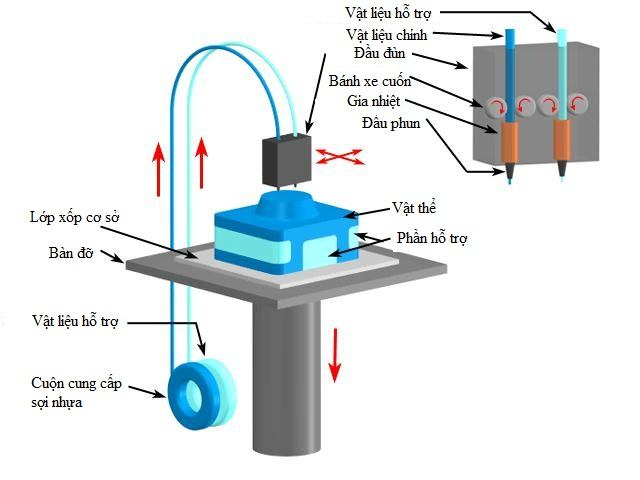
\includegraphics[scale=0.5]{images/nguyen-ly-fdm.jpg}
\caption{Cấu tạo và nguyên lý hoạt động của FDM}
\end{figure}

\begin{figure}[ht]
\centering
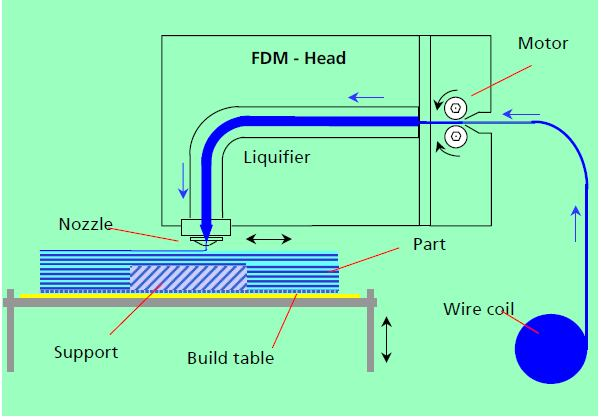
\includegraphics[scale=0.5]{images/so-do-nguyen-ly-fdm.jpg}
\caption{Sơ đồ nguyên lý FDM}
\end{figure}

\subsection{Ưu và nhược điểm}
\underline{\textit{Ưu điểm:}}\\
Là công nghệ in 3D giá rẻ, dễ sửa chữa và thay thế chi tiết máy móc, in với số lượng lớn, ít tốn nguyên liệu. Thường sử dụng trong các sản phẩm cần chịu lực. Tốc độ tạo hình 3D nhanh. Quá trình tạo mẫu nhanh của FDM không giống như công nghệ SLA, LOM, SLS phải sử dụng tia laser để tạo hình sản phẩm mà công nghệ tạo mẫu nhanh FDM đơn giản hơn rất nhiều, độ tin cậy cao, bảo dưỡng dễ dàng.

Công nghệ tạo mẫu nhanh FDM sử dụng vật liệu nhựa nhiệt dẻo không độc, không mùi, và do đó sẽ không gây ô nhiễm môi trường xung quanh. Thiết bị hoạt động tạo ra ít tiếng ồn.

\underline{\textit{Nhược điểm:}}\\
Ít khi dùng trong lắp ghép vì độ chính xác không cao. Khả năng chịu lực không đồng nhất .

\subsection{Phạm vi ứng dụng}
FDM được sử dụng khá rộng rãi trong thị trường in 3D nói chung vì giá thành rẻ, một trong những ứng dụng chính của công nghệ này là:
\begin{enumerate}
\item Tạo các mô hình mẫu
\item Chế tạo các bộ phận chi tiết nhỏ
\item Sử dụng được nhiều dạng vật liệu sinh học
\end{enumerate}

\section{Một số hình ảnh các máy in 3D ở công ty}
Công ty sử dụng nhiều máy in FDM để nhận phục vụ in 3D cho khách hàng, cũng như in các linh kiện để lắp ráp thêm các máy in 3D khác, một số hình ảnh của máy in 3D FDM ở công ty được tôi chụp lại trong quá trình thực tập có thể được xem ở hình \ref{img:3d_printer1} và \ref{img:3d_printer2}.

\begin{figure}[!ht]
\centering
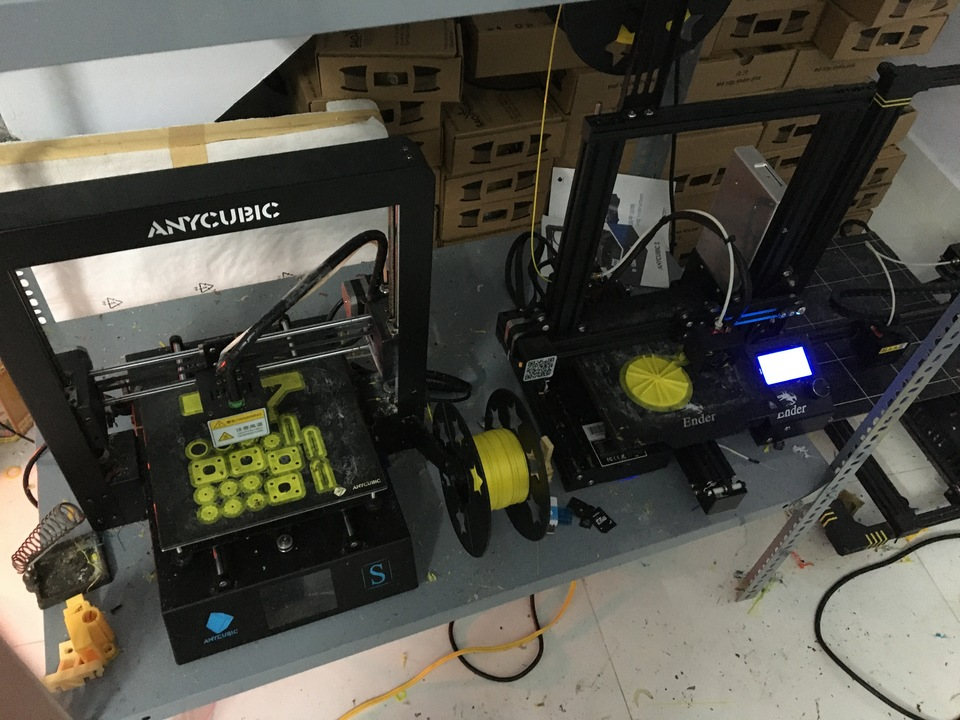
\includegraphics[scale=0.4]{images/img_0365_resized.jpg}
\caption{Hai máy in FDM đang hoạt động}
\label{img:3d_printer1}
\end{figure}

\begin{figure}[!ht]
\centering
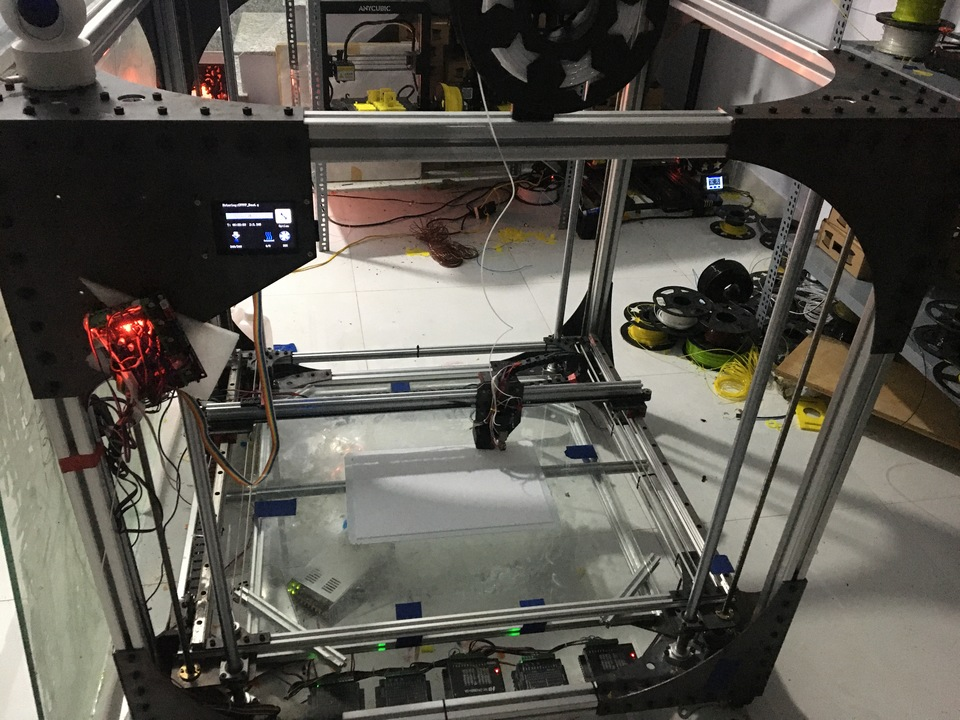
\includegraphics[scale=0.4]{images/img_0367_resized.jpg}
\caption{Máy in FDM khổ lớn đang hoạt động}
\label{img:3d_printer2}
\end{figure}

Công ty cũng bán loại mục in 3D PLA+ chất lượng cao, thân thiện môi trường với giá cả cực kì cạnh tranh trên thị trường, một hình ảnh về hai cuộn nhựa in 3D PLA+ có thể được xem ở hình \ref{img:3d_pla}.

Ngoài ra, công ty còn cung cấp nhiều mẫu mực in màu khác, người đọc có thể tham khảo tại website chính thức của công ty ở đường link: \url{https://nhuain3d.vn/}

\begin{figure}[!ht]
\centering
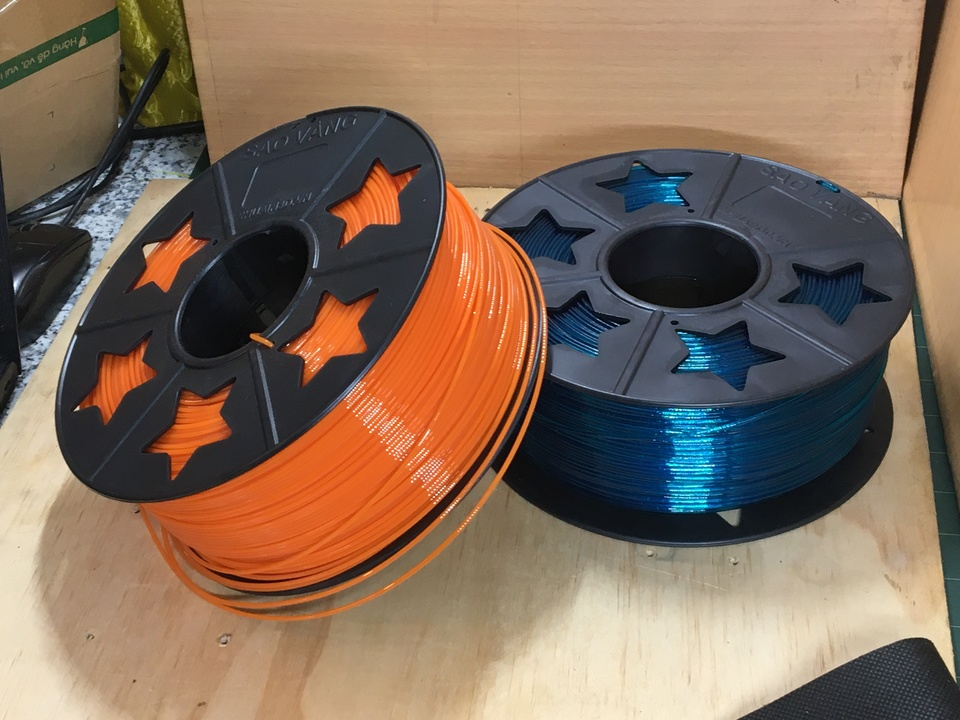
\includegraphics[scale=0.4]{images/img_0315_resized.jpg}
\caption{Hai mẫu cuộn nhựa in 3D PLA+ do công ty bán}
\label{img:3d_pla}
\end{figure}

Công ty cũng thực hiện lắp ráp máy in 3D mới để bán ra thị trường, một số hình ảnh về các mẫu sản phẩm đang được lắp ráp có thể xem ở các hình \ref{img:3d_printer_khung}, \ref{img:3d_printer_assembling} và \ref{img:3d_printer_fixing} 

\begin{figure}[!ht]
\centering
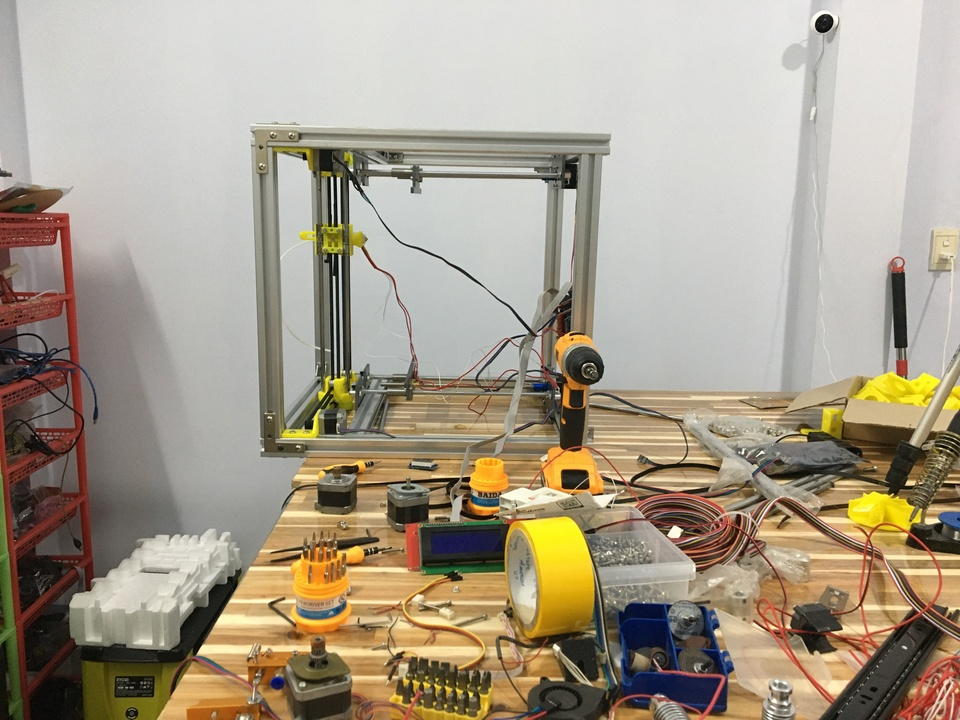
\includegraphics[scale=0.4]{images/img_0366_resized.jpg}
\caption{Một khung máy in 3D}
\label{img:3d_printer_khung}
\end{figure}

\begin{figure}[!ht]
\centering
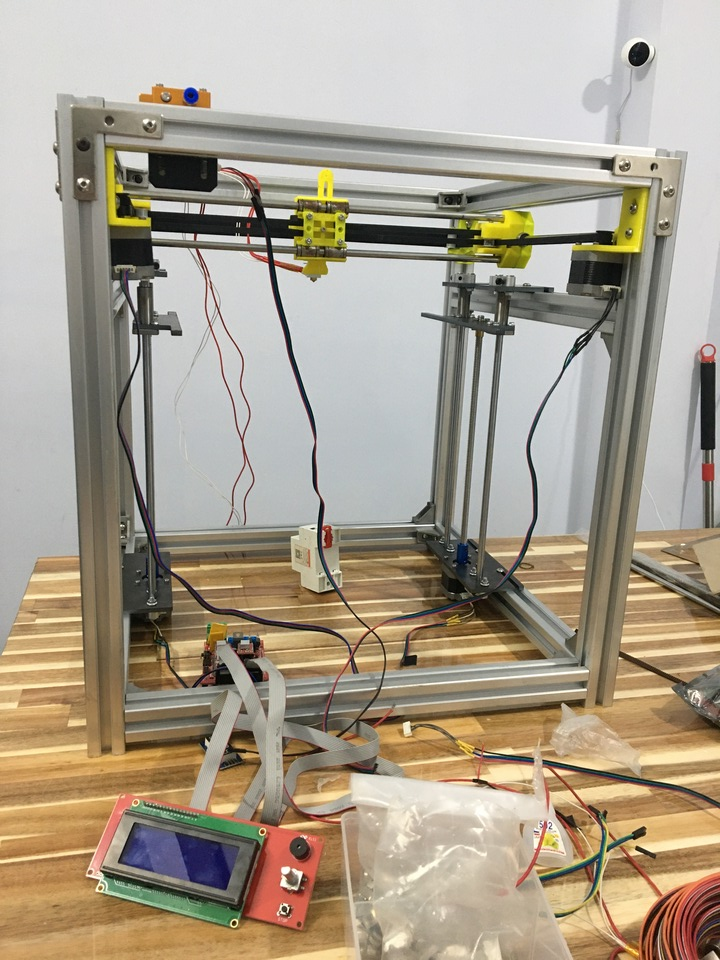
\includegraphics[scale=0.3]{images/img_0372_resized.jpg}
\caption{Máy in 3D đang được lắp ráp}
\label{img:3d_printer_assembling}
\end{figure}

\begin{figure}[!ht]
\centering
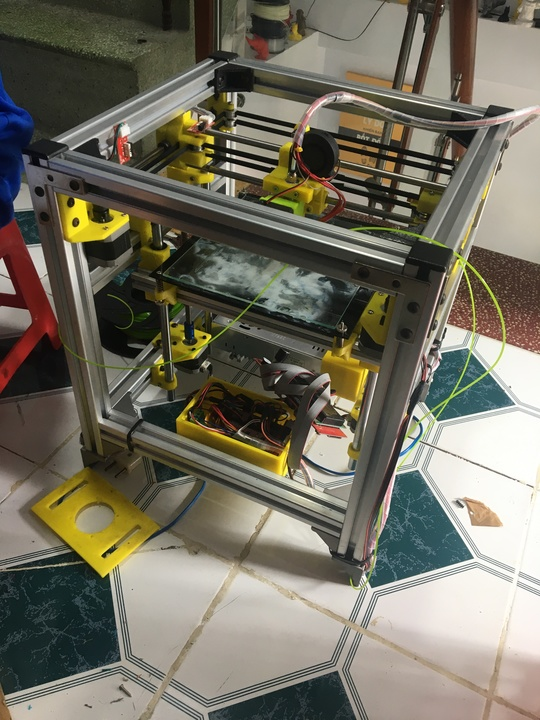
\includegraphics[scale=0.4]{images/img_0364_resized.jpg}
\caption{Máy in 3D đang được sửa chữa}
\label{img:3d_printer_fixing}
\end{figure}

Một số sản phẩm in 3D có thể được tham khảo ở các hình \ref{img:3d_print_prod1} và \ref{img:3d_print_prod2}.

\begin{figure}[!ht]
\centering
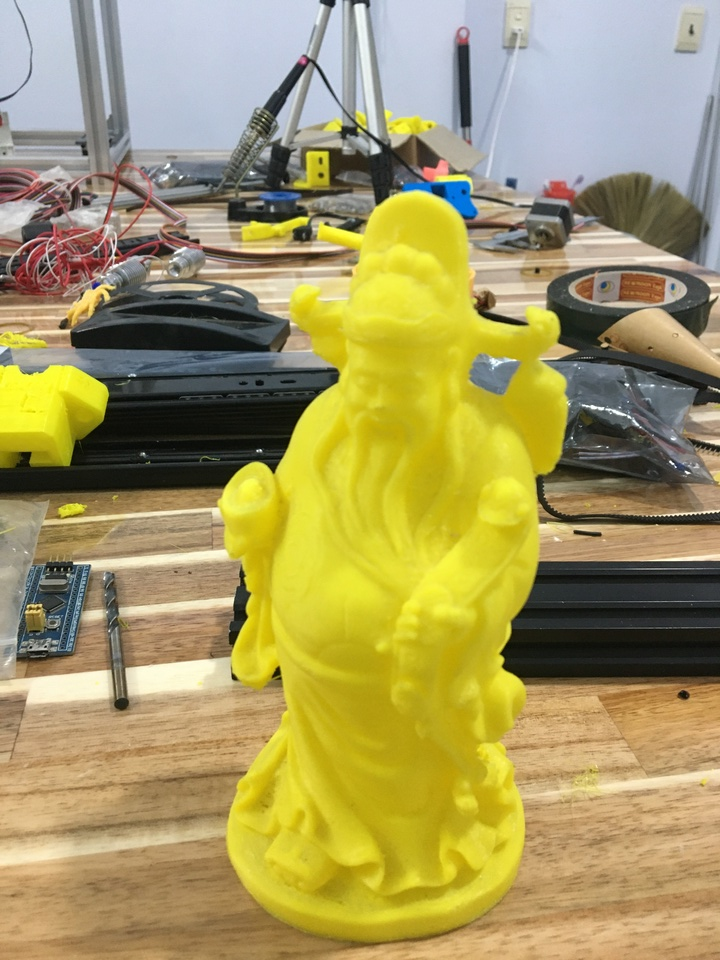
\includegraphics[scale=0.3]{images/img_0371_resized.jpg}
\caption{Một sản phẩm thử nghiệm in 3D}
\label{img:3d_print_prod1}
\end{figure}

\begin{figure}[!ht]
\centering
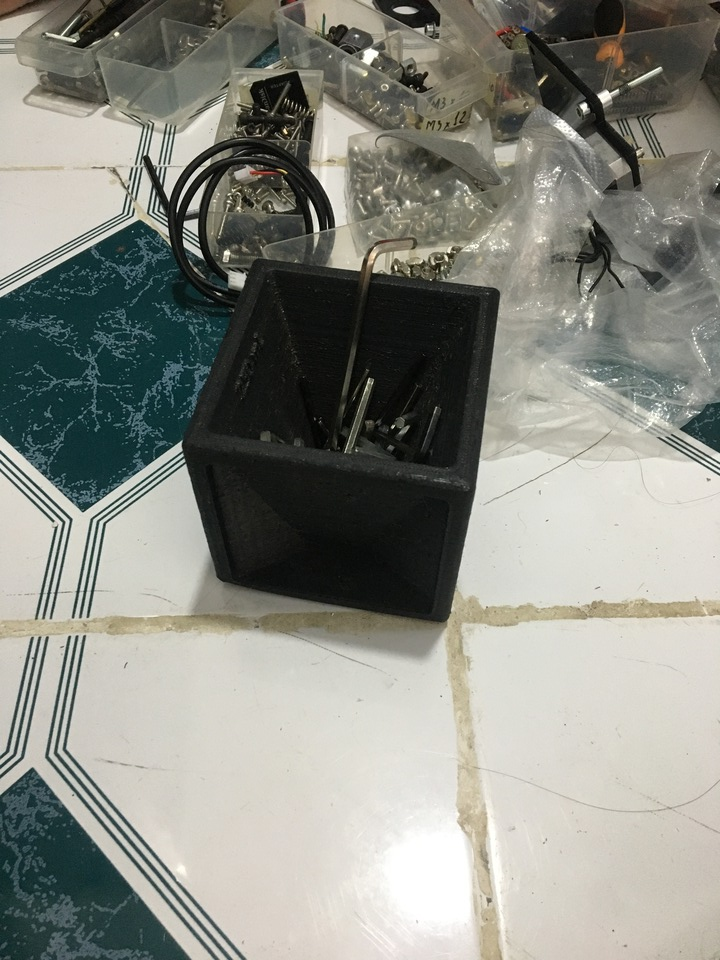
\includegraphics[scale=0.3]{images/img_0370_resized.jpg}
\caption{Một sản phẩm in 3D được dùng để chứa dụng cụ}
\label{img:3d_print_prod2}
\end{figure}

\section{Tìm hiểu lập trình STM8103F3F6 trên môi trường Linux}
\subsection{Tìm hiểu phần cứng}
STM8 là dòng vi điều khiển 8-bit cho hãng ST instrument sản xuất với giá thành rẻ và khả năng tiết kiệm điện năng vượt trội, thích hợp để nghiên cứu và ứng dụng trong hệ thống nhỏ, dùng pin và tối ưu chi phí.

STM8F3F6 vẫn có tương đối đầy đủ các chức năng và kết nối cơ bản như ADC, UART, I2C, SPI, v.v.. khá phù hợp với việc thực hiện nghiên cứu lập trình cho những người mới khởi đầu học lập trình nhúng.

Phần lớn các dòng vi điều khiển lập trình khác như 8051, PIC hay AVR đã có nhiều người thực hiện nghiên cứu về nó trước nên với một kit STM8103F3F6 nhỏ gọn sử dụng chip ARM thì đây là một lựa chọn để học cách làm việc độc lập, đọc tài liệu cho kĩ năng lập trình nhúng rất phù hợp.

\begin{figure}[!ht]
\centering
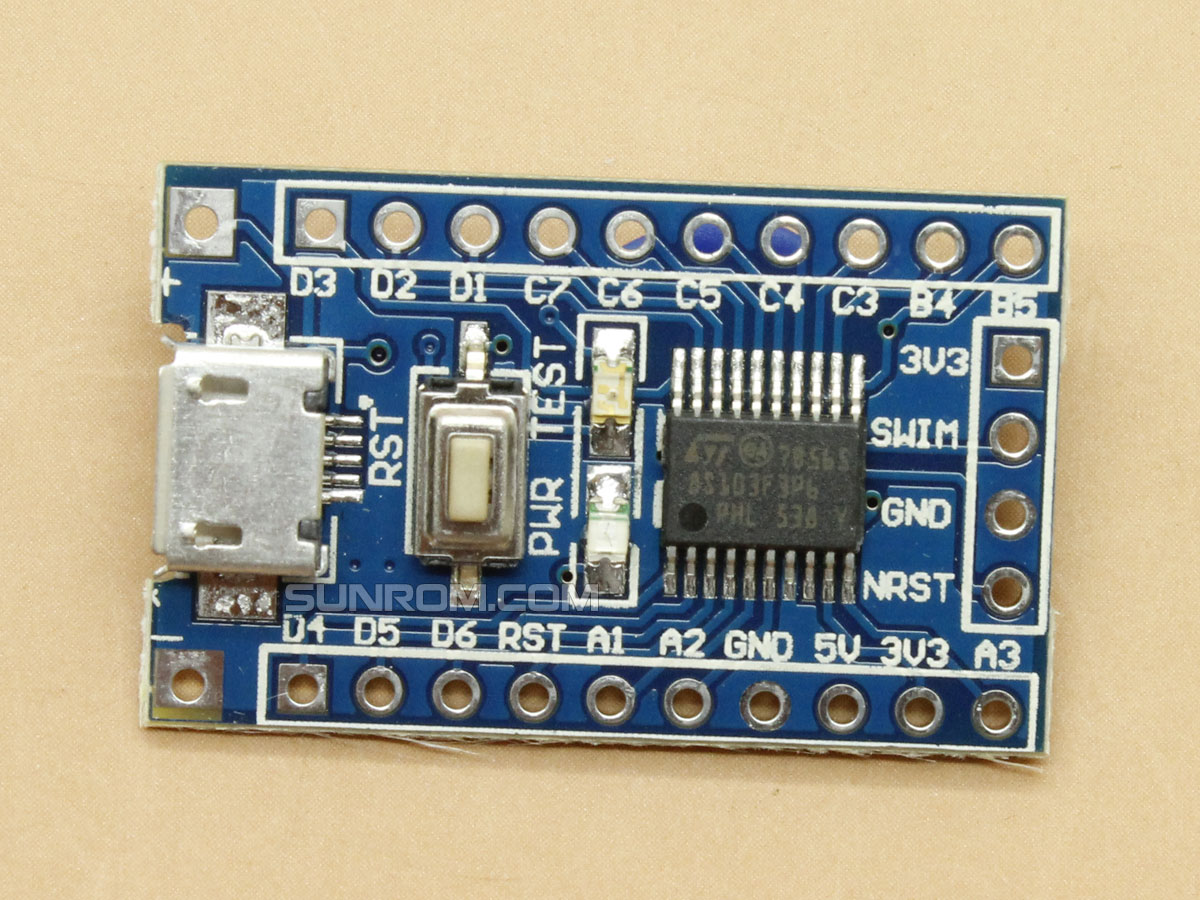
\includegraphics[scale=0.2]{images/stm8sf3f6.jpg}
\caption{Hình ảnh một kit STM8103F3F6 nhỏ gọn}
\end{figure}

STM8S103F3F6 là vi điều khiển 8 bit thuộc dòng Medium-desity, nghĩa là có dung lượng bộ nhớ lập trình được ở mức trung bình.
Cụ thể một số thông số như sau:

\begin{itemize}
\item Tốc độ tối đa 16 MHz.
\item Bộ nhớ:\\
    -- 8 KB bộ nhớ Flash\\
    -- 640 byte EEPROM \\
    -- 1 KB RAM
\item Clock và quản lý năng lượng\\
    -- Điện áp làm việc: từ 2.95V đến 5V.\\
    -- Điều khiển xung đồng lồ linh hoạt với 4 nguồn dao động\\
    -- Một số tính năng khác như low-power, switch-off.
\item Quản lý ngắt\\
    -- Bộ điều khiển ngắt lồng nhau tối đa 32 nguồn ngắn.\\
    -- 23 ngắt ngoài trên 6 vector
\item Timer: 8-bit timer, bộ prescaler 8-bit.
\item Các giao diện khác: UART, SPI, I2C.
\end{itemize}

\subsection{Môi trường lập trình Linux}
Rõ ràng là không có ai lập trình trực tiếp trên vi điều khiển cả, mà người lập trình sẽ viết mã, biên dịch, sửa lỗi trên máy tính trước rồi nạp chương trình xuống board mạch.
Vì vậy, lựa chọn một môi trường làm việc trên máy tính phù hợp có thể sẽ đẩy nhanh tốc độ phát triển của hệ thống.
Ở đây, tôi chọn môi trường hệ điều hành Linux, vì nó có sẵn nhiều bộ công cụ hỗ trợ cho việc lập trình ngôn ngữ C như \emph{gcc}, \emph{gdb}, v.v..

Và một lý do khác là nếu xảy ra lỗi trong quá trình lập trình trên môi trường này, người lập trình sẽ tự phải tìm hiểu cách sửa lỗi, từ đó học thêm được nhiều kinh nghiệm quý giá.

\subsection{Các công cụ khác}
\subsubsection{Thiết bị nạp ST-Link}
Mạch nạp STM8, STM32 ST-Link được sử dụng để nạp chương trình và debug cho vi điều khiển STM8 và STM32 của hãng ST instrument, mạch nạp có kích thước nhỏ gọn, chi phí thấp, độ bền cao.

Mạch có thể nạp sử dụng các chuẩn JTAG, SWD và SWV.

\begin{figure}[!ht]
\centering
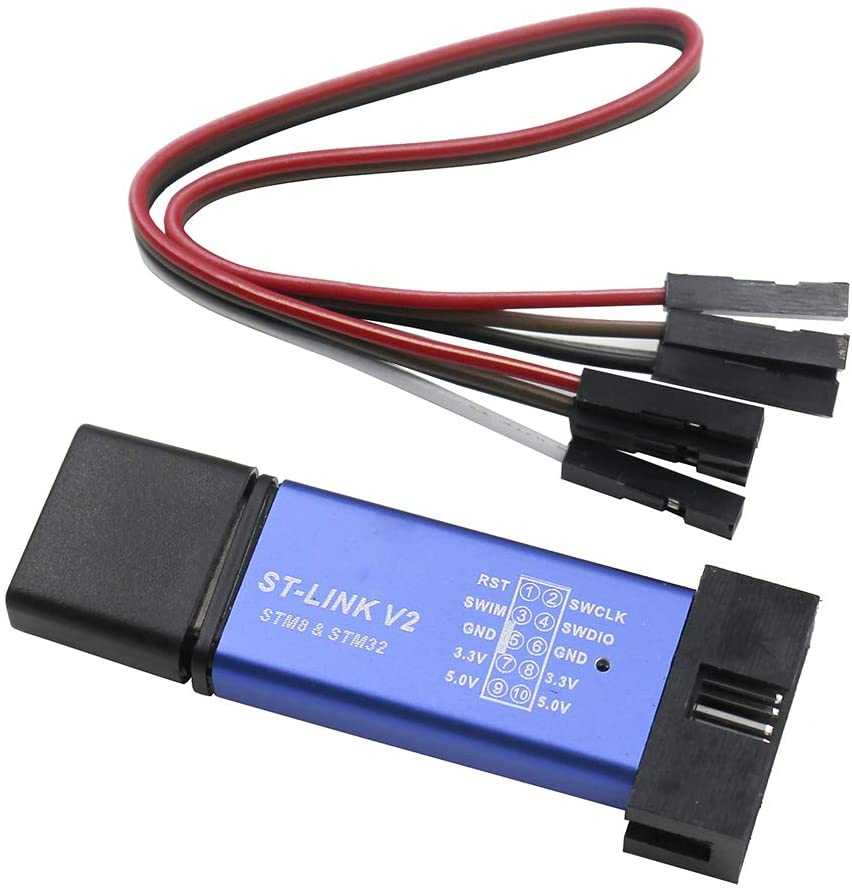
\includegraphics[scale=0.3]{images/st-link-v2.jpg}
\caption{Mạch nạp ST-Link V2}
\end{figure}

\subsubsection{Small Device C Compiler (SDCC)}
Small Device C Compiler (SDCC), là một trình dịch ngôn ngữ C cho rất nhiều họ vi điều khiển tới từ nhiều nhà sản xuất khác nhau, trong đó cũng có STM8.
Để tải về SDCC, hãy truy cập đến trang đại diện của SDCC tại địa chỉ https://sourceforge.net/projects/sdcc/,
download và làm theo hướng dẫn cài đặt trong tệp tin INSTALL.txt.
Một cách khác đơn giản hơn, chúng ta có thể sử dụng repository chính thức của Debian.

\mintinline{bash}{$ sudo apt install sdcc*}

SDCC cũng kèm theo tài liệu hướng dẫn người dùng, người đọc có thể tham khảo tại đường link: \url{http://sdcc.sourceforge.net/doc/sdccman.pdf} để hiểu rõ hơn cách sử dụng công cụ này.

\subsubsection{Make}
Make là công cụ build tự động được sử dụng phổ biến trong phát triển ứng dụng nguồn mở.
Ưu điểm của việc sử dụng Make là tính linh hoạt trong triển khai.
Với Make, bạn có thể biên dịch các chương trình hoàn toàn tự động mà không cần đến sự hỗ trợ của các IDE.
Có thể nhiều người cho rằng điều này không thiết thực lắm vì các công cụ hiện nay đã có thừa các chức năng tương tự.

Thông thường, Make được kèm theo phần lớn trong các distro của Linux.
Để kiểm tra đã cài đặt Make và phiên bản của nó hay chưa, ta chỉ cần gọi lệnh:
\begin{minted}{text}
$ make -v
GNU Make 4.1
Built for x86_64-pc-linux-gnu
Copyright (C) 1988-2014 Free Software Foundation, Inc.
License GPLv3+: GNU GPL version 3 or later <http://gnu.org/licenses/gpl.html>
This is free software: you are free to change and redistribute it.
There is NO WARRANTY, to the extent permitted by law.
\end{minted}

\subsubsection{stm8flash}
Chương trình \emph{stm8flash} được sử dụng để nạp code đã biên dịch xuống board.
Ta có thể cài đặt stm8flash từ repo này: \url{https://github.com/vdudouyt/stm8flash}.

\subsection{Thư viện ngoại vi tiêu chuẩn}
Các vi điều khiển STM8 của ST được cung cấp một bộ giao diện lập trình ứng dụng (API) có tên là STM8 Standard Peripheral Library (STM8-SPL).

Thư viện tiêu chuẩn này cung cấp đủ các thao tác cơ bản trong quá trình sử dụng.
Một số chức năng nâng cao thì người lập trình sẽ tự viết giao diện interface phù hợp với dự án phát triển riêng.
Ta có thể tải thư viện STM8-SPL (với một số thay đổi để phù hợp với việc sử dụng chung với SDCC) tại repo: \url{https://github.com/bschwand/STM8-SPL-SDCC/}

Có một số thay đổi cần phải lưu ý đó là:\\
-- Thư viện gốc do ST cung cấp chỉ hoạt động với bộ compiler của nhà sản xuất, vì vậy cần phải thay đổi một số định nghĩa của các header để có thể sử dụng với SDCC.\\
-- SDCC chỉ có thể tối ưu hóa theo từng module chứ không phải từng hàm trong một module, vì vậy ta cần phải chia các hàm ra thành các module nhỏ hơn trong thư viện để SDCC có thể tối ưu hóa các hàm này.\\
-- Thư viện trong đường liên kết trên đã bao gồm một Makefile tuong đối hoàn chỉnh để tiện cho việc phát triển kit STM8 trên môi trường Linux.

Cấu tạo của thư viện STM8-SPL tương tự như hình \ref{img:SPL_structure}.

\begin{figure}[!ht]
\dirtree{%
.1 STM8 Standard Peripheral Library.
.2 \_htmresc.
.3 logo.bmp.
.2 Libraries.
.3 STM8S\_StdPeriph\_Driver.
.4 inc.
.4 src.
.2 Project.
.3 STM8S\_StdPeriph\_Examples.
.3 STM8S\_StdPeriph\_Template.
.2 Ultilities.
.3 STM8S\_EVAL.
.2 MCD-ST Liberty SW License Agreement V2.pdf.
.2 Release\_Notes.html.
.2 stm8s-a\_stdperiph\_lib\_um.chm.
}
\caption{Cấu trúc của STM8-SPL}
\label{img:SPL_structure}
\end{figure}

\pagebreak
Một số điểm đáng lưu ý trong thư viện này là:
\begin{itemize}
\item Thư mục Libraries, bên trong là thư mục con STM8S\_StdPeriph\_Driver.
    Đây chính là bộ thư viện của chúng ta.
    Thư mục inc lưu trữ các tệp tin header, thư mục src là mã nguồn của các header tương ứng.
    Mỗi một ngoại vi sẽ có một header file và một source file đi kèm.
    Ví dụ, thư viện cho GPIO sẽ có header file là stm8s\_gpio.h nằm trong thư mục inc và source file là stm8s\_gpio.c nằm trong thư mục src.
    Trong thư mục inc có một tệp đặc biệt không có source tương ứng, đó là stm8s.h.
    Đây là nơi định nghĩa tất cả các địa chỉ thanh ghi, bit thanh ghi, bản đồ bộ nhớ, tần số thạch anh, v.v..
\item Thư mục Project/STM8S\_StdPeriph\_Examples chứa bên trong những thư mục con là các ví dụ cơ bản về sử dụng một thư viện tương ứng với tên của thư mục con đó.
    Ví dụ, EXTI sẽ có các ví dụ về sử dụng thư viện ngắt ngoài (External Interrupt – sử dụng thêm hai file stm8s\_exti.h và stm8s\_exti.c).
    Và thư mục Project/STM8S\_StdPeriph\_Template chứa một khuôn mẫu dự án tiêu chuẩn do ST cung cấp để người lập trình tham khảo, thường để tham khảo cho việc lập trình trên môi trường Windows sử dụng STVD-Cosmic, Raisonance hoặc IAR.
\item Thư mục Utilities/STM8S\_EVAL: là thư viện khai báo thêm cho cái kit STM8/128 EVAL (dùng STM8S2xx).
    Vì đề tài này thực hiện nghiên cứu STM8S103F3F6 nên thư mục này thực sự không có nhiều lợi ích, tuy nhiên có ba thư viện về LCD1602, giao tiếp SD card qua SPI và EEPROM qua I2C nếu chỉnh sửa có thể sử dụng được trực tiếp.
\item Tệp tin stm8s-a\_stdperiph\_lib\_um.chm: là hướng dẫn sử dụng của bộ thư viện, trong đó giải thích đầy đủ nội dụng của toàn bộ các thư mục, danh sác hàm, các cấu trúc (struct), các định nghĩa (define),v.v.. trong các tệp tin để người phát triển có thể làm việc thuận tiện hơn.
\end{itemize}

Trong liên kết tải thư viện STM8-SPL đã được chỉnh sửa ở trên đã bao gồm các file Makefile với nội dung biên dịch mã nguồn C cho kit STM8.
Có một thay đổi nhỏ cần lưu ý khi sử dụng file này đó là: ở phiên bản SDCC 3.9, công cụ \emph{sdar} đã chính thức thay thế cho công cụ cũ là \emph{sdcclib}.
Vì vậy, nếu người dùng sử dụng các phiên bản SDCC mới thì cần thay đổi tệp \mintinline{text}{Libraries/STM8_StdPeriph_Driver/Makefile} ở các dòng sau:\\
-- Dòng 25: \mintinline{text}{AR = sdcc} thành \mintinline{text}{AR = sdar}.\\
-- Dòng 84: \mintinline{text}{$(AR) -a $(TARGET) $^} thành \mintinline{text}{$(AR) -rc $(TARGET) $^}.

Ngoài ra, ta có thể thay đổi Makefile để flash trực tiếp từ máy tính sang board sử dụng Makefile bằng cách thêm hai dòng sau vào cuối Makefile:
\begin{minted}{text}
flash: $(TARGET)
        stm8flash -c stlinkv2 -p stm8s103f3 -s flash -w $<
\end{minted}

\section{Thực hiện lập trình một số ngoại vi cơ bản}
\subsection{GPIO}
\textbf{Giới thiệu chung}:\\
General Purpose Input/Output (GPIO) là khối chức năng cơ bản với mọi loại vi điều khiển, nắm vai trò tương tác với bên ngoài.
Một port I/O gồm tối đa 8 chân.
Mỗi chân có thể được lập trình riêng là một đầu vào kỹ thuật số (digital input) hoặc đầu ra kỹ thuật số (digital output).
Ngoài ra, một số port có thể có chức năng thay thế (alternative function – AF) như đầu vào tương tự (ADC), ngắt ngoài (EXTI), đầu vào / đầu ra cho ngoại vi trên chip.
Chỉ có một chức năng thay thế có thể được ánh xạ tới một chân tại một thời điểm, việc ánh xạ chức năng thay thế được điều khiển bởi byte tùy chọn.

Một thanh ghi dữ liệu đầu ra, thanh ghi dữ liệu đầu vào,thanh ghi hướng dữ liệu và hai thanh ghi cấu hình có liên quan tới mỗi port.
Một chân cụ thể sẽ hành xử như một đầu vào hoặc đầu ra phụ thuộc vào trạng thái của thanh ghi dữ liệu hướng của port.

\bigskip
\textbf{Thực hiện lập trình GPIO cho STM8}:

Chương trình đầu tiên cũng là chương trình cơ bản nhất là thực hiện nháy LED ở chân PB5 (là chân nối với LED trên board) có thể xem ở ví dụ \ref{code:gpio_example}.
\begin{listing}[!ht]
\begin{ccode}
#include "stm8s.h"
#include "stm8s_it.h"    /* SDCC patch: required by SDCC for interrupts */

#define LED_GPIO_PORT  (GPIOB)

void main(void)
{

  /* Initialize I/Os in Output Mode */
  GPIO_Init(LED_GPIO_PORT, GPIO_PIN_5, GPIO_MODE_OUT_PP_LOW_FAST);

  while (1)
  {
    /* Toggles LEDs */
    GPIO_WriteReverse(LED_GPIO_PORT, GPIO_PIN_5);
    Delay(0xFFFF);
  }
}

void Delay(uint16_t nCount)
{
  /* Decrement nCount value */
  while (nCount != 0)
  {
    nCount--;
  }
}

#ifdef USE_FULL_ASSERT

void assert_failed(uint8_t* file, uint32_t line)
{
  /* User can add his own implementation to report the file name and line number,
     ex: printf("Wrong parameters value: file %s on line %d\r\n", file, line) */

  /* Infinite loop */
  while (1)
  {
  }
}
#endif
\end{ccode}
\caption{Chương trình GPIO cơ bản -- nháy LED}
\label{code:gpio_example}
\end{listing}

\pagebreak
\subsection{Điều khiển đồng hồ trên STM8}
\textbf{Giới thiệu chung}:\\
Cũng như các mạch tích hợp đồng bộ khác, STM8S cũng yêu cầu nguồn cấp xung đồng hồ để hoạt động.
Nguồn cấp xung đồng hồ trên dòng vi điều khiển này có thể xuất phát từ 3 nguồn khác nhau, gồm 2 nguồn dao động nội là LSI (tốc độ thấp -- 128kHz), HSI (tốc độ cao -- 16MHz) và một nguồn dao động bên ngoài tốc độ cao HSE (giá trị dao động từ 1 – 16MHz với STM8S và tối đa 24 MHz trên dòng STM8AF).
Nhìn chung thì các nguồn dao động nội trên STM8S có thể đáp ứng tương đối tốt những công việc cơ bản (trong những ví dụ đầu tiên chẳng hạn).
Tuy nhiên, đây đều là các mạch dao động RC, về lâu về dài, độ chính xác trong hoạt động không thể đảm bảo.
HSE, với nguồn cấp lấy từ thạch anh hoặc các thiết bị tạo dao động sẽ là lựa chọn tin cậy hơn.

\begin{figure}[ht]
\centering
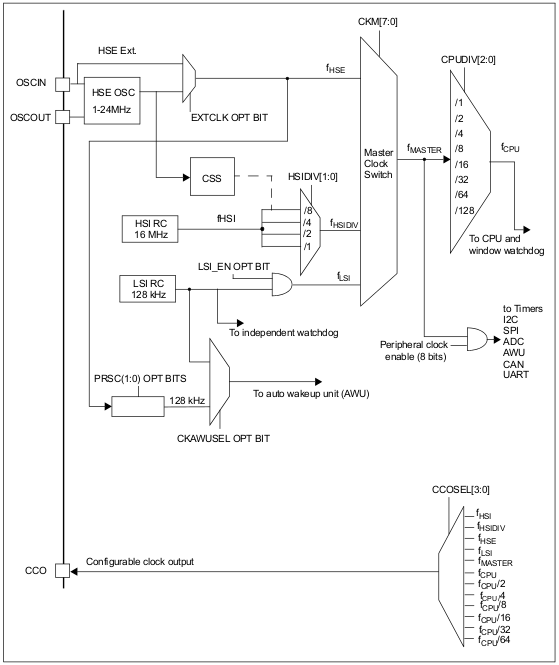
\includegraphics[scale=0.5]{images/clock_tree.png}
\caption{Cấu tạo khối quản lý xung đồng hồ trên STM8}
\end{figure}

\textbf{Cấu hình sử dụng thư viện SPL}:\\
Cấu hình trên vi điều khiển và lập trình - ở đây chỉ giới thiệu về tập lệnh sử dụng trong thư viện SPL, không đi sâu vào thanh ghi.
Người đọc có nhu cầu tìm hiểu về thanh ghi có thể xem thêm manual của chip (Reference manual RM00016).

Chế độ mặc định của STM8S là sử dụng HSI với clock/8 khi chưa cấu hình gì.
Cấu hình clock với mode HSI:
\begin{listing}
\begin{ccode}
void CLK_Configuration(void)
{
    CLK_DeInit();
    CLK_HSIPrescalerConfig(CLK_PRESCALER_HSIDIV1); // HSI voi ty le chia 1
    // 16 Mhz/1 = 16 Mhz
}
\end{ccode}
\caption{Cấu hình đồng hồ với mode HSI}
\end{listing}

\pagebreak
Cấu hình clock sử dụng thạch anh ngoài (HSE) mode automatic:
\begin{listing}
\begin{ccode}
void CLK_Configuration(void)
{
    CLK_DeInit();
    CLK_HSECmd(ENABLE); // Enable HSE
    while(CLK_GetFlagStatus(CLK_FLAG_HSERDY) != SET); // wait till HSE is ready
    CLK_ClockSwitchConfig(CLK_SWITCHMODE_AUTO, CLK_SOURCE_HSE, DISABLE, CLK_CURRENTCLOCKSTATE_DISABLE);
    while(CLK_GetSYSCLKSource() != CLK_SOURCE_HSE);
    CLK_ClockSwitchCmd(DISABLE);
    CLK_SYSCLKConfig(CLK_PRESCLAER_CPUDIV1); // PRESCALER DIV 1
}
\end{ccode}
\caption{Cấu hình đồng hồ sử dụng HSE với mode automatic}
\end{listing}

Nhìn chung, việc chuyển đổi giữa các nguồn xung đồng hồ cũng như thay đổi tốc độ đồng hồ trên STM8S khá đơn giản, chỉcần hiểu và cấu hình hợp lý các bộ chọn kênh trong khối điều khiển clock là đã có thể thực hiện điều này.

\subsection{Ngắt trên STM8}
\textbf{Giới thiệu chung}:\\

Để làm việc với ngắt trong STM8S, nhà sản xuất đưa ra khối ITC (interrupt controller).
Khối ITC quản lý tất cả các loại ngắt xảy ra trên vi điều khiển, bao gồm:
\begin{itemize}
\item Quản lý ngắt phần cứng
    -- Các khả năng gây ngắt ngoài trên đa số các chân I/O với vector ngắt chuyên dụng và thiết lập sườn (cạnh) gây ngắt trên mỗi cổng.\\
    -- Các khả năng gây ngắt trên ngoại vi.
\item Quản lý ngắt mềm (TRAP)
\item Quản lý ngắt lồng nhau hoặc đồng thời với cấp độ và mức độ ưu tiên linh hoạt:
    -- Lên đến 4 mức ngắt lồng nhau có thể lập trình được.\\
    -- Lên đến 32 vector ngắt gán cố định bởi phần cứng.\\
    -- 2 sự kiện ngắt không che được: RESET, TRAP.\\
    -- 1 ngắt phần cứng top level không che được (TLI).
\end{itemize}

Một danh sách ngắn gọn để tiện tham khảo có thể xem tham khảo ở bảng sau:
\begin{longtable}{lll}
\textbf{Chỉ số} & \textbf{Nguồn gây ngắt} & \textbf{Mô tả}\\
\midrule
\endhead
--- & RESET & Reset \\
--- & TRAP & Software interrupt \\
0 & TLI & External top level interrupt \\
1 & AWU & Auto wake up from halt \\
2 & CLK & Clock controller \\
3 & EXTI0 & Port A external interrupt \\
4 & EXTI1 & Port B external interrupt \\
5 & EXT2 & Port C external interrupt \\
6 & EXT3 & Port D external interrupt \\
7 & EXT4 & Port E external interrupt \\
10 & SPI & End of transfer \\
11 & TIM1 & Timer 1 update/overflow/underflow/trigger/break \\
12 & TIM1 & Timer 1 capture/compare \\
13 & TIM2 & Timer 2 update/overflow \\
14 & TIM2 & Timer 2 capture/compare \\
17 & UART1 & Tx complete \\
18 & UART1 & Receive register DATA FULL \\
19 & I2C & I2C interrupt \\
22 & ADC1 & ADC1 end of conversion/analog watchdog interrupt \\
23 & TIM4 & Timer 4 update/overflow \\
24 & Flash & EOP/WR\_PG\_DIS \\
\bottomrule
\caption{Danh sách vector ngắt STM8S103F3F6}
\label{tbl:stm8s_interrupts}
\end{longtable}

Về vấn đề độ ưu tiên, trên STM8 có 2 dạng ưu tiên ngắt là ưu tiên phần mềm (lập trình được) và ưu tiên phần cứng.
Khi có ngắt xảy ra đồng thời, ngắt nào có độ ưu tiên phần mềm cao hơn sẽ được thực hiện mà không bận tâm đến mức độ ưu tiên phần cứng.
Khi các ngắt có mức ưu tiên phần mềm tương đương nhau, mức độ ưu tiên phần cứng được dùng đến để sắp xếp thứ tự phục vụ.
Địa chỉ vector ngắt cố định nằm tại vùng địa chỉ cao trên bản đồ bộ nhớ (0x00 8004 đến 0x00 807C) được sắp xếp theo thứ tự ưu tiên phần cứng.
Mức độ ưu tiên phần mềm gồm 4 mức được mô tả ở bảng \ref{tbl:int_priority} dưới, được lưu theo 2 bit trong các thanh ghi ITC\_SPRx.
Lưu ý, các vector ngắt không thể thiết lập mức ưu tiên mềm bằng 0.

\begin{longtable}{cccc}
\textbf{Ưu tiên} & \textbf{Mức ưu tiên} & \textbf{I0} & \textbf{I1}\\
\midrule
\endhead
Mức 0 (main) & Mức cao nhất & 1 & 0 \\
Mức 1 & Thấp hơn mức 0 & 0 & 1 \\
Mức 2 & Thấp hơn mức 1 & 0 & 0 \\
Mức 3 (Không ngắt phần mềm) & Mức thấp nhất & 1 & 1 \\
\bottomrule
\caption{Mức độ ưu tiên ngắt phần mềm}
\label{tbl:int_priority}
\end{longtable}

Hai chế độ quản lý ngắt:

\begin{itemize}
\item Ngắt đồng thời: tất cả các ngắt có ưu tiên mềm ở mức 3, ngoại trừ TLI, RESET, TRAP. Đây là chế độ mặc định sau khi reset vi điều khiển.
\item Ngắt lồng nhau: chế độ này cho phép gián đoạn trong khi đang phục vụ một ngắt khác. Chế độ được kích hoạt khi có bất cứ ngắt nào được thiết mức ưu tiên mềm nhỏ hơn 3.
\end{itemize}

Về ngắt ngoài, trên STM8S105 có tất cả 5 vector ngắt ngoài:

\begin{itemize}
\item 5 tuyến trên Port A: PA[6:2]
\item 8 tuyến trên Port B: PB[7:0]
\item 8 tuyến trên Port C: PC[7:0]
\item 7 tuyến trên Port D: PD[6:0]
\item 8 tuyến trên Port E: PE[7:0]
\end{itemize}

PD7 là nguồn Top Level Interrupt (TLI).
Để tạo ra một ngắt, cổng GPIO tương ứng phải được cấu hình trong chế độ đầu vào với các ngắt được kích hoạt.
Các bạn tham khảo các mô tả thanh ghi trong chương GPIO – tài liệu hướng dẫn tham chiếu hoặc bài viết trước để biết chi tiết.
Sườn nhạy ngắt phải được cấu hình trong thanh ghi EXTI\_CR1 và EXTI\_CR2.

\textbf{Trình phục vụ ngắt}:\\
SDCC cho phép viết thủ tục dịch vụ ngắt trong C, với một số từ khóa mở rộng.
\begin{ccode}
void some_isr (void) __interrupt (1)
{
...
}
\end{ccode}

Các số tùy chọn sau từ khóa \_\_interrupt là chỉ số của vector ngắt (trong ví dụ trên là 1).
Trình biên dịch sẽ chèn thêm một lời gọi đến trình phục vụ (ở ví dụ này là hàm some\_isr) trong bảng vector ngắt theo chỉ số đã định.
Nếu có nhiều file nguồn trong dự án, trình phục vụ có thể có mặt trong bất kỳ tệp tin nào, nhưng một prototype của chúng phải được khai báo hoặc bao hàm (\#include) trong tập tin \emph{main.c}.

\textbf{Một ví dụ về ngắt ngoài}:\\
Chương trình sau thực hiện ngắt ngoài để điều khiển nháy LED, sử dụng LED ngoài được nối với chân PD7.

Để thực hiện điều này, ta sử dụng hai tệp đó là tệp main.c chứa chương trình chính và tệp stm8s\_it.c chứa phần mã điều khiển khi xảy ra ngắt.
Ở tệp tin main.c, chúng ta bao hàm thư viện một số thư viện:
\begin{itemize}
\item stm8s.h: tệp định nghĩa thanh ghi và ánh xạ bộ nhớ
\item stm8s\_it.h: tệp định nghĩa nguyên mẫu các trình phục vụ ngắt
\item stm8s\_itc.h: tệp định nghĩa nguyên mẫu các hàm thư viện ITC
\item stm8s\_exti.h: tệp định nghĩa nguyên mẫu các hàm thư viện ngắt ngoài
\item stm8s\_gpio.h: tệp định nghĩa nguyên mẫu các hàm thư viện GPIO
\end{itemize}

\begin{ccode}
#include "stm8s.h"
#include "stm8s_it.h"
#include "stm8s_itc.h"
#include "stm8s_exti.h"
#include "stm8s_gpio.h"

int EXTI_config(void);
int GPIO_config(void);

static void Delay(uint32_t t)
{
 while(t--);
}

int EXTI_config(void) {
  /* De-initialized external interrupt */
  EXTI_DeInit();
  /* External interrupt port D block, falling edge */
  EXTI_SetExtIntSensitivity(EXTI_PORT_GPIOD, EXTI_SENSITIVITY_FALL_ONLY);
  /* Enable interrupts */
  enableInterrupts();

  return 0;
}

int GPIO_config(void) {
  /* De-initialized GPIOD */
  GPIO_DeInit(GPIOD);
  /* Initialized PD7 as output, low frequency operation */
  GPIO_Init(GPIOD, GPIO_PIN_7, GPIO_MODE_OUT_PP_LOW_FAST);
  /* Initialized PD6 as input, pull-up & external interrupt */
  GPIO_Init(GPIOD, GPIO_PIN_6, GPIO_MODE_IN_PU_IT);

  return 0;
}

int main( void )
{
  /* GPIO config */
  while(GPIO_config());
  /* External interrupt config */
  while(EXTI_config());

  while(1)
  {
  /* Wait interrupt event occur */
    Delay(5);
  }
}

#ifdef USE_FULL_ASSERT

void assert_failed(uint8_t* file, uint32_t line)
{
  (void)file;
  (void)line;
  /* User can add his own implementation to report the file name and line number,
  ex: printf("Wrong parameters value: file %s on line %d\r\n", file, line) */

  /* Infinite loop */
  while (1)
  {
  }
}
#endif
\end{ccode}

\pagebreak
Sau đó ta chỉnh sửa tệp tin \emph{stm8s\_it.c}, tìm tới trình phục vụ ngắt của port D và thay đổi như sau:
\begin{listing}
\begin{ccode}
...
INTERRUPT_HANDLER(EXTI_PORTD_IRQHandler, 6)
{
  if((GPIOD->IDR && GPIO_PIN_6) == 0x00)
  {
    GPIO_WriteReverse(GPIOD, GPIO_PIN_&);
  }
}
...
\end{ccode}
\caption{Chương trình stm8s\_it.c cho ngắt ngoài}
\end{listing}

\chapter{Tổng kết công việc thực tập}
\section{Kết quả thực tập}
Trên đây là những lý thuyết mà tôi đã nghiên cứu và học được trong quá trình nghiên cứu về cách lập trình trên kit STM8S103F3F6 trong thời gian thực tập tương đối ngắn tại công ty.
Có thể nói rằng, kit STM8S103F3F6 là một đối tượng vi điều khiển rất phù hợp cho việc học tập và nghiên cứu cho người bắt đầu học lập trình nhúng.
Tuy phần nghiên cứu trên còn thiếu nhiều lý thuyết như sử dụng UART, ADC hay đặc biệt là tính năng One-wire bus của kit tuy nhiên tôi đã học được rất nhiều phần mềm mã nguồn mở lý thú như \emph{SDCC}, \emph{Makefile} hay cách cài đặt, chỉnh sửa và sử dụng thư viện SPL do hãng ST cung cấp.

Qua quá trình thực tập, tôi cũng đã học được nhiều hiểu biết cơ bản về các hệ thống sử máy móc cũng như là công nghệ in FDM cho việc in các sản phẩm 3D.
\section{Nhận xét}
Trong quá trình thực tập, tôi đã tích lũy được nhiều kiến thức, kĩ năng thiết thực về hướng ngành Lập trình nhúng trong bộ môn Điện tử -- Viễn thông, cũng như là những kiến thức ngoài về in 3D qua các công việc được giao ở công ty.
Những kiến thức này tạo tiền để tôi có nhận thức đúng đắn hơn về ngành nghề mà mình đã chọn lựa, cũng như là kim chỉ định hướng cơ bản cho quá trình thực hiện luận văn.
Các công việc được giao cũng đã tăng cường khả năng vận dụng kiến thức đã học vào thực tiễn, khả năng tìm kiếm và tự nghiên cứu đọc tài liệu, rèn luyện phương pháp làm việc hiệu quả, báo cáo tiến độ công việc và các kỹ năng mềm trong môi trường làm việc công nghiệp.

%\include{content/ch3-ketqua}

\backmatter
\phantomsection
\addcontentsline{toc}{chapter}{Tài liệu tham khảo}
\nocite{*} % Basically don't cite anything but print all of the stuff in bibliography file out
\emergencystretch=1em
\printbibliography[title=Tài liệu tham khảo]
% This is the default way to handle bibliography
%\bibliographystyle{ieeetr}
%\bibliography{uni}

%----- APPENDIX (PHU LUC) -----
% Detailed schematic, extra information, source code and other shit are put in here
%\appendix
%\chapter*{Phụ lục}
%\addcontentsline{toc}{chapter}{Phụ lục}
%% IMPORTANT: These have to be here, cannot put above else it would mess up the content in mainmatter
%\renewcommand{\thesection}{\Alph{section}}
%%\setminted[c]{linenos, breaklines, breakanywhere, fontsize=\footnotesize]
%\section{Source code của hệ thống}
%\subsection{Thư viện MFRC522}
%\subsubsection{File header}
%\inputminted[linenos=true, breaklines, breakanywhere, fontsize=\footnotesize]{cpp}{code/Mfrc522.h}
%\subsubsection{File thư viện}
%\inputminted[linenos=true, breaklines, breakanywhere, fontsize=\footnotesize, encoding=utf8]{cpp}{code/Mfrc522.cpp}
%\subsection{Thư viện LCD}
%\subsubsection{File header}
%\inputminted[linenos=true, breaklines, breakanywhere, fontsize=\footnotesize]{c}{code/lcd.h}
%\subsubsection{File thư viện}
%\inputminted[linenos=true, breaklines, breakanywhere, fontsize=\footnotesize]{c}{code/lcd.c}
%\subsection{File main}
%\inputminted[linenos=true, breaklines, breakanywhere, fontsize=\footnotesize]{c}{code/main.c}
\end{document}
